% !Mode\dots ``TeX:UTF-8''
% !TEX root = ../bare_jrnl.tex

\section{Algorithms for online observability}
\label{sec:deter}
To  determine  online observability of \BCN s, one needs to determine $\Ks(\Ded(\mathcal{S}_\BB,\varepsilon,\mathsf{o}(0)))$ for every non-empty $\Ded(\mathcal{S}_\BB,\varepsilon, \mathsf{o}(0))$. 

%\subsection{Input-labelled graph}
We start with input-labelled graph $\mathcal{G}=(\mathcal{V}, \mathcal{E}, \mathcal{L})$.

\begin{definition}[Input-labelled Graph]
Let $\mathcal{V}$, $\mathcal{E}$ and $\mathcal{L}$ be the vertex set, the edge set and the labelling function of an input-labelled graph $\mathcal{G}=(\mathcal{V}, \mathcal{E}, \mathcal{L})$. $\mathcal{G}$ is called the input-labelled graph of the \BCN\, if 
\begin{itemize}
\item  $\mathcal{V}=\{\mathsf{S}\in\bigcup_{j=0}^{(2^{n} -1)} 2^{\Ded(\mathcal{S}_\BB,\varepsilon,\delta^j_{2^{n}} )}|\ \Ks(\mathsf{S})\ne \infty\}$;
\item  $\mathcal{E}=\{(\mathsf{S}_1,\mathsf{S}_2)\in \mathcal{V}\times \mathcal{V}|$ $\mathsf{S}_2\in\{\Ded(\mathsf{S}_1,\mathsf{i},\mathsf{o})|\mathsf{i}\in\Ri(\mathsf{S}_1),\mathsf{o}\in  \mathcal{O}\}\}$;
\item  $\mathcal{L}:\mathcal{E}\mapsto 2^{\Delta_L}=(\mathsf{S}_1,\mathsf{S}_2)\mapsto\{\mathsf{i}\in \Ri(\mathsf{S}_1)|\mathsf{S}_2\in\{\Ded(\mathsf{S}_1,\mathsf{i},\mathsf{o})|\mathsf{o}\in  \mathcal{O}\}\}$.
 \end{itemize}
\end{definition}

\begin{figure}[thpb]
      \centering
      \framebox{\parbox{3in}{
		\centerline{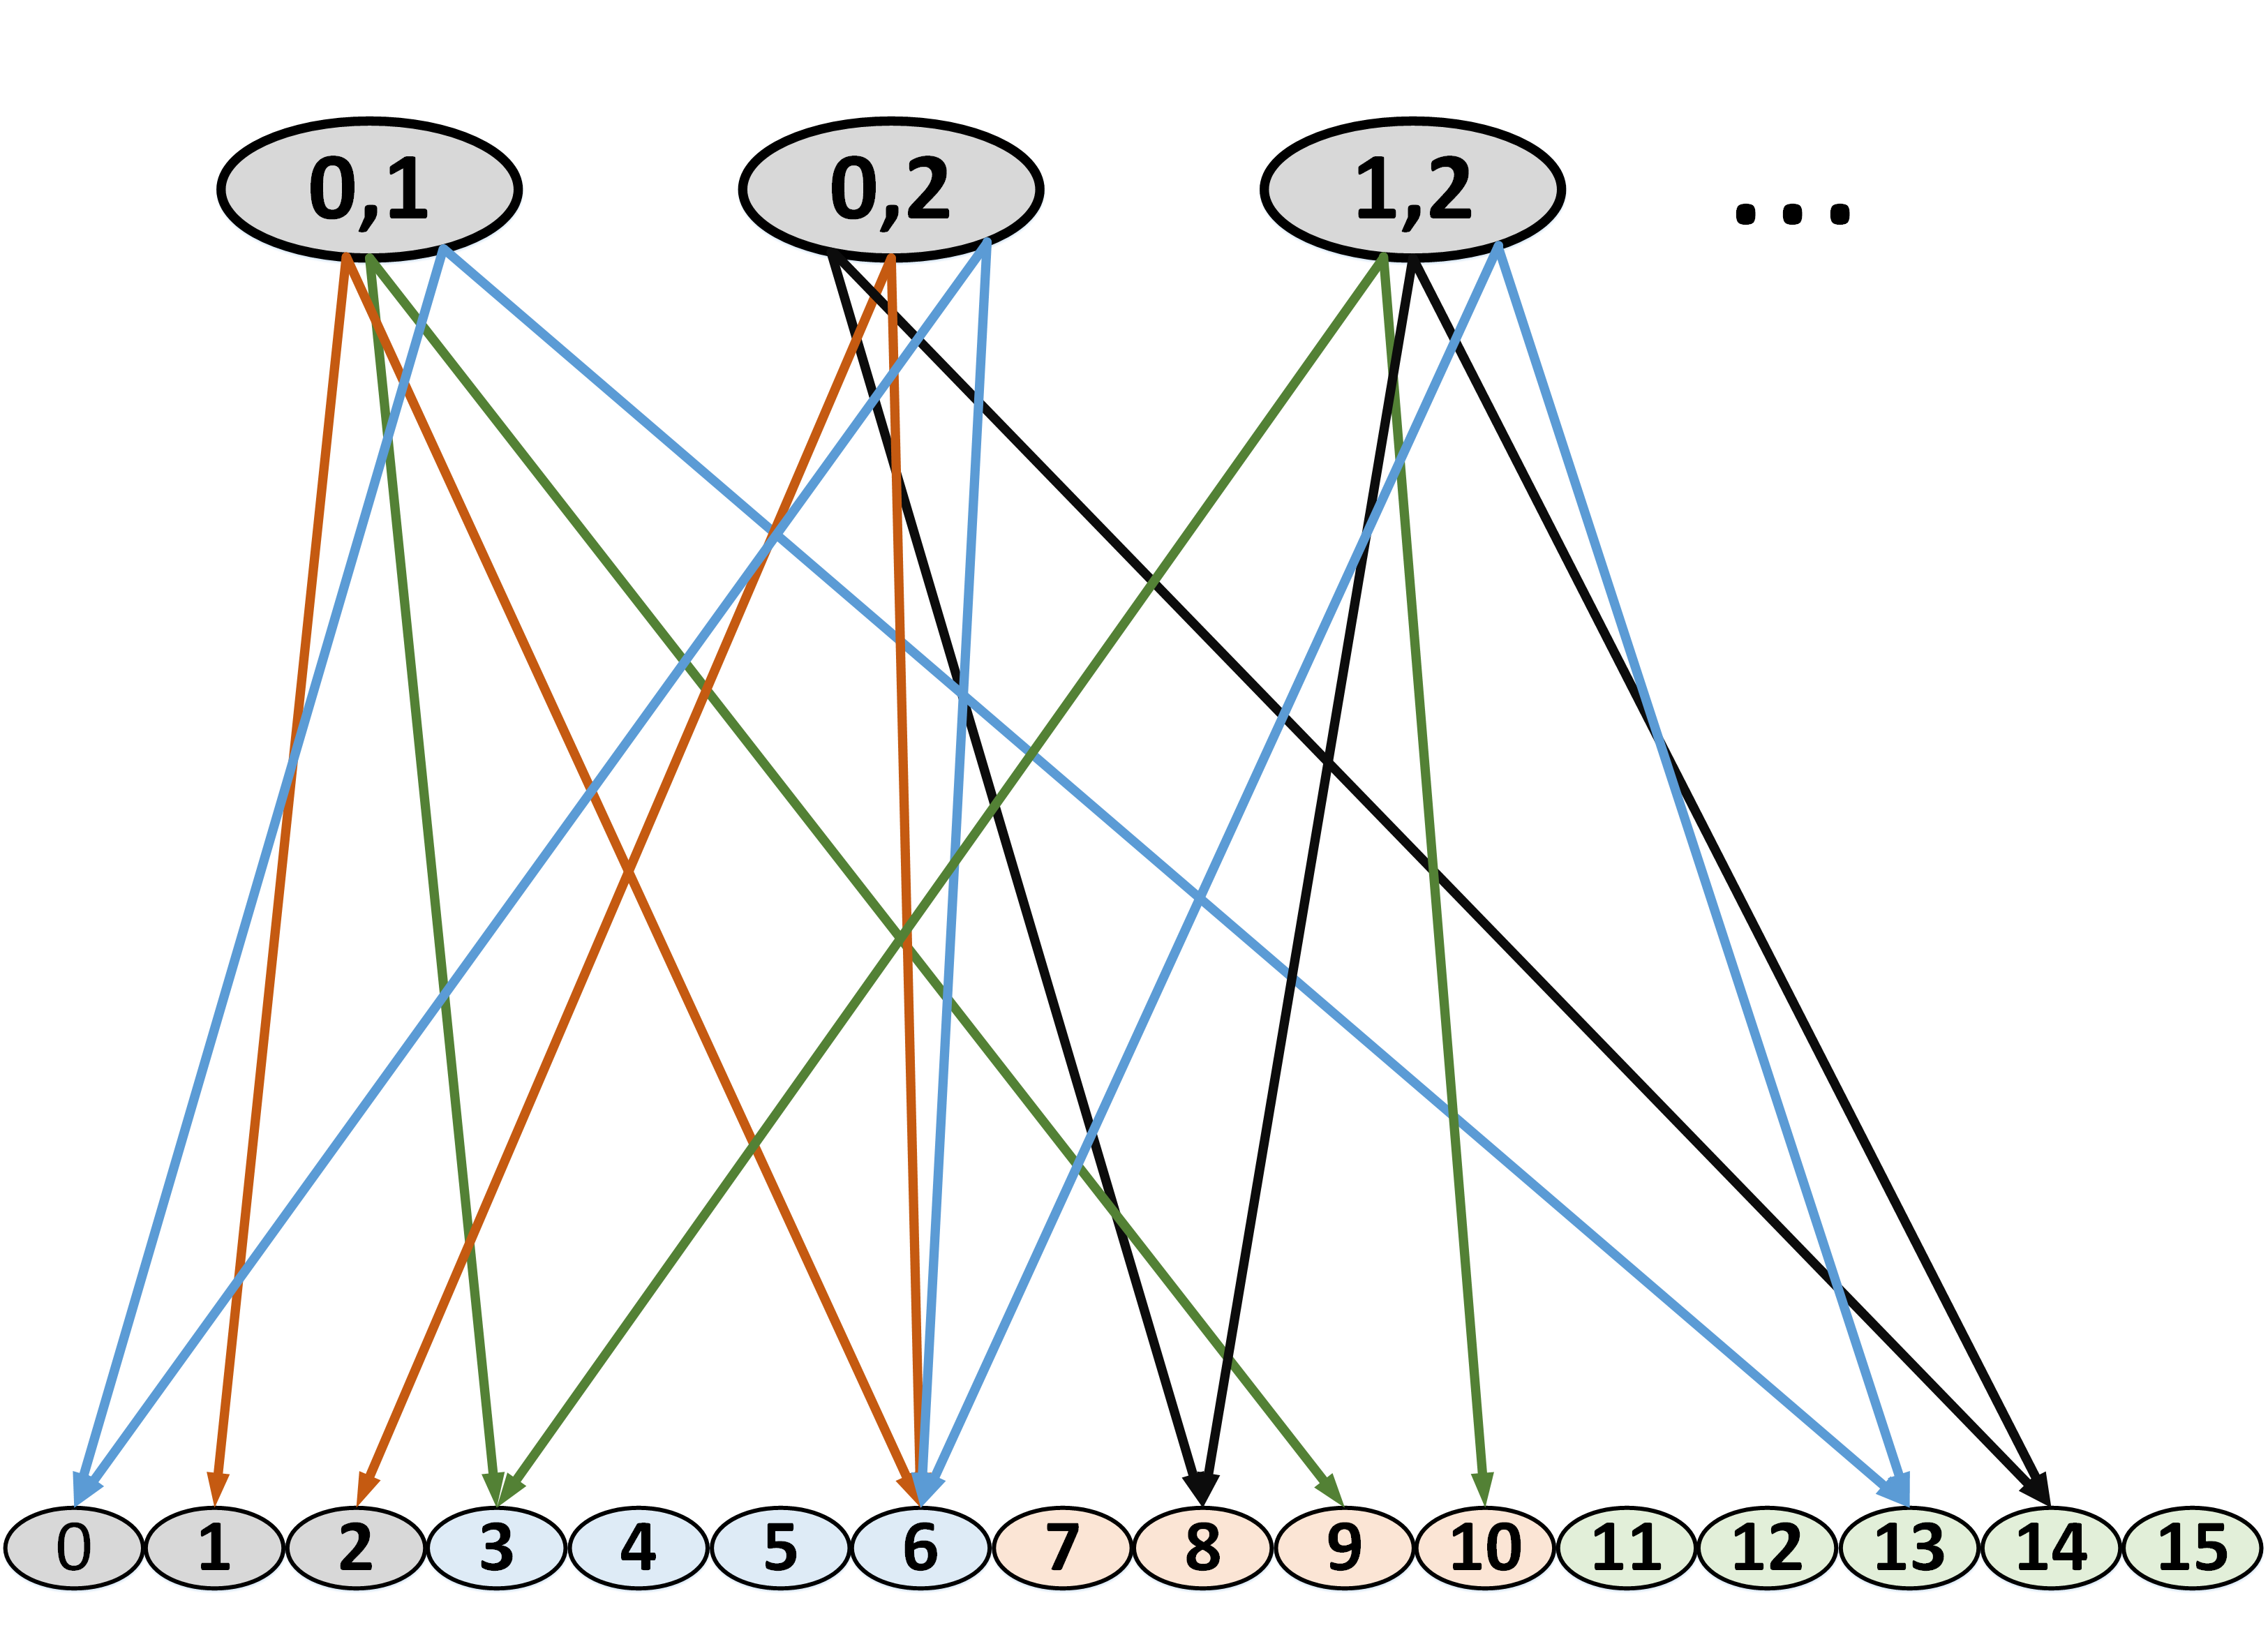
\includegraphics[scale=0.090]{figures/Fig4.png}}
	}}
      \caption{Part of the input-labelled graph, where the green, black, orange, blue edges are labelled with $\{\delta_4^0\}$, $\{\delta_4^1\}$, $\{\delta_4^2\}$ and $\{\delta_4^3\}$ respectively.}
      \label{fig:4}
\end{figure}
Intuitively, $\mathcal{V}$ represents a set of the state sets that for every $\mathsf{S}\in \mathcal{V}$, $\Ks(\mathsf{S})\ne \infty$ and for every $\mathsf{s}\in\mathsf{S}$, $\mathsf{s}$ produces the same output. $\mathcal{E}$ represents the relationship between the state sets which belong to $\mathcal{V}$, and $\mathcal{L}$ labels every $\mathsf{e} \in\mathcal{E}$ with a set of inputs. %Then, based on the definition of the input-labelled graph, we have a \BCN\ is online observable iff every non-empty $\Ded(\Delta_M,\varepsilon, \mathsf{o}^{j}(0))\in \mathcal{V}$.%Thus we can determine $\Ks(\Ded(\Delta_N,\varepsilon,\mathsf{o}^{j}(0)))$ of every non-empty $\Ded(\Delta_N,\varepsilon, \mathsf{o}^{j}(0))$ by checking the input-labelled graph.

%From the {\em Lemma \ref{lemm:1}}, we have that if for the set of states $\mathsf{S}^1$ there does not exist any $k^{1}\ge 0$ such that $\mathsf{S}^{1}$ is $k^{1}$-step determinable, and $\mathsf{S}^{1}\subseteq \mathsf{S}^{2}$. Then there does not exist any $k^{2}\ge 0$ that make $\mathsf{S}^{2}$ $k^{2}$-step determinable. Therefore, i

% \subsection{Determination algorithm}
With the input-labelled graph $\mathcal{G}=(\mathcal{V}, \mathcal{E}, \mathcal{L})$, we have a \BCN\ $\BB$ is online observable iff every non-empty $\Ded(\mathcal{S}_\BB,\varepsilon, \mathsf{o}(0))\in \mathcal{V}$.
 Then, we propose the {\bf Algorithm~\ref{alg:1}} to determine the online observability. That, we construct the input-labelled graph, and check whether every non-empty $\Ded(\mathcal{S}_\BB,\varepsilon, \mathsf{o}(0))\in \mathcal{V}$.
 
 In the process of constructing the input-labelled graph for a \BCN\ $\BB$, we construct the vertexes which consist of a smaller number of states before constructing the vertexes which consist of a greater number of states.
\begin{itemize}
\item  Because, once we find a $\mathsf{S}$ that $\Ks(\mathsf{S})= \infty$, i.e. $\mathsf{S}\notin \mathcal{V}$, and as there exists $\mathsf{o}\in \mathcal{O}$, such that $\mathsf{S}\subseteq \Ded(\mathcal{S}_\BB,\varepsilon, \mathsf{o})$, we have $\Ks(\Ded(\mathcal{S}_\BB,\varepsilon, \mathsf{o}))= \infty$, i.e. $\Ded(\mathcal{S}_\BB,\varepsilon, \mathsf{o}(0))\notin \mathcal{V}$ based on the {\em Lemma \ref{lemm:1}}, i.e. the \BCN\ $\BB$ is not online observable.
\item  And we can determine the scope of $\Ri(\mathsf{S})$ if we have determined $\Ri(\mathsf{S}')$ for every $\mathsf{S}'\subset\mathsf{S}$ based on the {\em Lemma \ref{lemm:2}}. With the scope of $\Ri(\mathsf{S})$ we can determine the $\Ks(\mathsf{S})$ more easily.
 \end{itemize} %, and it can find all paths to determine $\mathsf{s}(0)$ if the \BCN\ is online observable.

\begin{algorithm}[h]
\caption{Determination algorithm}
\begin{algorithmic}[1]
\REQUIRE 
The updating rules of a \BCN
\ENSURE  
The input-labelled graph of this \BCN
\STATE Boolean value $Ob=$ true 
\STATE integer $i$ , $j$, $z=1$\
\STATE array $VertexArray[\ ]$, $InputArray[\ ]$
\STATE {\sf constructvertex}($z$)
\STATE $VertexArray=${\sf constructvertex}($++z$)
\WHILE {($VertexArray!=$Null)}
\FOR{($i=0$; $i<arraysize(VertexArray)$; $i++$)}
\IF{($z==2$)}
\STATE $InputArray$ = $\mathcal{I}_\BB$ 
\ELSE

\STATE $InputArray$=$\bigcap^{\mathsf{S}\in VertexArray[i]} \Ri(\mathsf{S})$ 
\ENDIF
\FOR{($j=0$; $j<arraysize(InputArray)$; $j++$)}
\STATE Check $VertexArray[i]$ by $InputArray[j]$ 
\STATE Build edges for $VertexArray[i]$ 
\ENDFOR
\IF {($\Ri(VertexArray[i])=\emptyset$)}
\STATE  $Ob=$ false 
\STATE Return Null
\ENDIF
\ENDFOR
\STATE $VertexArray=${\sf constructvertex}($++z$)
\ENDWHILE
\STATE Return $\mathcal{S}_\BB$\
\end{algorithmic}
 \label{alg:1}
\end{algorithm}


\begin{algorithm}[h!]
\caption{{\sf constructvertex}(integer $z$)}
\begin{algorithmic}[1]
\REQUIRE 
The number of states $z$
\ENSURE  
The vertexes with $z$ states producing the same outputs 
\STATE  Construct all vertexes with $z$ states producing the same output 
\IF{(Failed to construct)} 
\STATE  Return Null
\ELSE 
\STATE  Classify these vertexes
\STATE Sort the states in these vertexes
\STATE Sort these vertexes
\STATE Return vertexes
\ENDIF 
\end{algorithmic}
 \label{alg:2}
\end{algorithm}

%Some details of {\bf Algorithm~\ref{alg:1}} and {\bf Algorithm~\ref{alg:2}}:
%\begin{itemize}
%\item Construct all vertexes with $z$ states producing the same outputs. For every non-empty $\Ded(\Delta_M,\varepsilon,\mathsf{o})$, if $z>|\Ded(\Delta_M,\varepsilon,\mathsf{o})|$, then we could not get any set from $\Ded(\Delta_M,\varepsilon,\mathsf{o})$, otherwise, we get $\frac{(|\Ded(\Delta_M,\varepsilon,\mathsf{o})|)!}{z!\times (|\Ded(\Delta_M,\varepsilon,\mathsf{o})|-z)!}$ sets of states from $\Ded(\Delta_M,\varepsilon,\mathsf{o}^{j})$, where $z!$ is the factorial of $z$, and them construct vertexes by the sets of states. 

% \item Sort the states in these vertexes and sort these vertexes: We sort the states inside the vertexes at first, and then sort the vertexes by the states of them. For example, in Fig.~\ref{fig:4} the vertexes $\{\delta_{16}^0,\delta_{16}^1\}$, $\{\delta_{16}^0,\delta_{16}^2\}$ and $\{\delta_{16}^1,\delta_{16}^2\}$ are well shorted. 
 % \item Determine $InputArray$ by other vertexes:
 %  For a vertex $VertexArray[i]$ which consists of $z$ states, we use the vertexe which consists of the first $(z-1)$ states of $VertexArray[i]$ and the vertexe which consists of the last $(z-1)$ states of $VertexArray[i]$ to find $InputArray$ for $VertexArray[i]$. For example, from Fig.~\ref{fig:4}, we have $\Ri(\{\delta_{16}^0,\delta_{16}^1\})=\{\delta_{4}^0,\delta_{4}^2,\delta_{4}^3\}$ and $\Ri(\{\delta_{16}^1,\delta_{16}^2\})=\{\delta_{4}^0,\delta_{4}^1,\delta_{4}^3\}$. Then we can take the intersection of them to be $InputArray$ of $\{\delta_{16}^0,\delta_{16}^1,\delta_{16}^2\}$ i.e. $InputArray=\{\delta_{4}^0,\delta_{4}^3\}$. 
 % \item Check $VertexArray[i]$ by $InputArray[j]$. Check whether $InputArray[j]\in \Ri(VertexArray[i])$.

%\end{itemize} 


 If a \BCN\ $\BB$ with the online observability, then its initial state $\mathsf{s}(0)$ can be determined by followng procedures.

\begin{description}
	\item[Step 1]  Determine the set $\mathsf{S}(0)$ of possible valuations of initial state $\mathsf{s}(0)$ by the output $\mathsf{o}(0)$ of $\BB$, i.e. $\mathsf{S}(0)=\Ded\left(\mathcal{S}_\BB,\varepsilon,\mathsf{o}(0)\right)$, and set the set variable $\mathsf{S}=\mathsf{S}(0)$ by $\mathsf{S}(0)$.
	\item[Step 2] Input to the \BCN\ $\BB$ with an $\mathsf{i}\in\Ri(\mathsf{S})$, and run $\BB$ to generate the new output $\mathsf{o}(t)$. 
	\item[Step 3] Determine the new $\mathsf{S}(t)$ by the input $\mathsf{i}$, output $\mathsf{o}(t)$ and $\mathsf{S}$, i.e. $\mathsf{S}(t)=\Ded\left(\mathsf{S},\mathsf{i},\mathsf{o}(t)\right)$, and update the set $\mathsf{S}=\mathsf{S}(t)$ by $\mathsf{S}(t)$.
	\item[Step 4] If the cardinal number of $\mathsf{S}$ equals to $1$, then return $\mathsf{s}'(0)$ which determined by the output sequence $\mathsf{O}[t]=\mathsf{o}(0)\ldots\mathsf{o}(t)$ and input sequence $\mathsf{I}[t]=\mathsf{i}(0)\ldots\mathsf{i}(t-1)$ of $\BB$ as the initial state. %That is for the input sequence $\mathsf{I}[t]=\mathsf{i}(0)\ldots\mathsf{i}(t-1)$ of $\BB$,  the output sequence $\mathsf{O}'[t]=\mathsf{o}'(0)\ldots\mathsf{o}'(t)$ produced by $\mathsf{s}'(0)$ and $\mathsf{I}[t]$ equals to $\mathsf{O}[t]$.
	 Otherwise, go to Step 2.
\end{description}
%From the Step 2, we have for every $ k=1,\ldots, t$, for every $\mathsf{s}'(k)\in \mathsf{S}(k)$, there is only one corresponding $\mathsf{s}'(k-1)\in \mathsf{S}(k-1)$ such that the $\mathsf{s}'(k)$ is determined by $\mathsf{s}'(k-1)$ and $\mathsf{i}(k-1)$. Thus %once $|\mathsf{S}|=1$, we can determine $\mathsf{s}(t)$, and then determine $\mathsf{s}(t-1),\dots,\mathsf{s}(0)$.
  In Step 4, when $|\mathsf{S}|=1$, for the input sequence $\mathsf{I}[t]$, there is only one initial state $\mathsf{s}'(0)$ whose corresponding output sequence  $\mathsf{O}'[t]=\mathsf{o}'(0)\ldots\mathsf{o}'(t)$ equals to the output sequence $\mathsf{O}[t]$ of $\BB$, thus, we can determine the initial state by $\mathsf{I}[t]$ and $\mathsf{O}[t]$. 

 From the {\em Example \ref{exa:10}}, we have the \BCN\ mentioned in {\em Example \ref{exa:2}} does not satisfies the {\bf Type-III} observability but its initial state $\mathsf{s}(0)$  can be determined without resetting. 
 This further illustrates that online observability is the necessary and sufficient condition of determining the initial state $\mathsf{s}(0)$ of a \BCN\  without  resetting.


%With the algorithm based on directed graph we can find all paths to determine the initial state of a \BCN. Thus, at time step $t$, we can use the $\mathsf{S}(t)$ and the directed graph to derive all of the input $\mathsf{i}(t)$ which can help us determine $\mathsf{s}(0)$. While, there comes a problem. Which input is the best input? To solve this problem, in the {\em Section \ref{sec:app}}, we will present how to decide the input to get better performance.
